\part*{Appendix}
\addcontentsline{toc}{chapter}{Appendix}
\setcounter{section}{0}
\renewcommand{\thesection}{\arabic{section}}
\renewcommand{\theHsection}{A.\arabic{section}}
\renewcommand{\theequation}{\arabic{equation}}
\setcounter{table}{0}
\renewcommand{\thetable}{A.\arabic{table}}
\renewcommand{\theHtable}{A.\arabic{table}}
\setcounter{figure}{0}
\renewcommand{\thefigure}{A.\arabic{figure}}
\renewcommand{\theHfigure}{A.\arabic{figure}}
\section{Set Covering Formulation}\label{app:set-covering}
Section~\ref{sec:fra-sp} introduces set covering (SC) as the fallback \gls{drispi} runs in place of set partitioning (SP) when the route pool does not yet cover every customer at least a minimum number of times. With $R$ the route pool at the time of the solve, $c_r$ the cost of route $r \in R$, $C$ the customer set of the instance (Section~\ref{sec:lit-problem}), $C_r \subseteq C$ the customer set of route $r$, and $x_r \in \{0, 1\}$ selecting route $r$, SC relaxes the partition equality of SP (Equation~\ref{eq:sp-partition}) to the cover inequality of \citet{garfinkelSetPartitioningProblemSetCovering1969}, who characterize set partitioning as set covering under an equality constraint:
\begin{align}
\text{min} \quad & \sum_{\mathclap{r \in R}} c_r x_r \label{eq:sc-obj}\\
\text{s.t.} \quad & \sum_{\mathclap{r \in R:\, i \in C_r}} x_r \geq 1, && \forall i \in C \label{eq:sc-cover}\\
& x_r \in \{0, 1\}, && \forall r \in R. \label{eq:sc-binary}
\end{align}
As with SP, \gls{drispi} solves the LP relaxation of Equation~\ref{eq:sc-binary}, $x_r \in [0, 1]$, first; the resulting fractional weights update the pool's quality scores in the same way regardless of whether the solve ends up running SC or SP, and the binary re-solve is warm-started from that relaxation.
\newpage
\section{XL Instance Detailed Results}\label{app:xl-results}
Table~\ref{tab:xl-summary} reports the per-instance detail underlying the Section~\ref{sec:stu-comparison} comparison: instance characteristics, \gls{drispi}'s best cost and gap to the current \gls{bks} for all 100 XL instances, alongside the initial-\gls{bks} and current-\gls{bks} reference costs.

% TODO(style): deviates from the "no shrinking below body size" rule in
% STYLE.md \S8; kept in portrait (rather than the rotating/sidewaystable
% default for wide tables) at the user's request, which requires scriptsize
% to fit twelve columns inside \textwidth.
\begin{scriptsize}
\setkomafont{caption}{\normalsize}
\setkomafont{captionlabel}{\normalsize}
\setlength{\tabcolsep}{3pt}
\begin{longtable}{@{}rlcllrrrrrrr@{}}
\caption{Instance-Level Best-of-3 Results for \gls{drispi} on the 100 XL Instances.}\label{tab:xl-summary}\\
\toprule
& & & & & & & \multicolumn{2}{c}{\gls{drispi}} & \multicolumn{2}{c}{Initial BKS} & \multicolumn{1}{c}{BKS} \\
\cmidrule(lr){8-9} \cmidrule(lr){10-11} \cmidrule(lr){12-12}
\# & Name & Dep & Cust & Dem & $Q$ & $r$ & \multicolumn{1}{c}{Cost} & Gap (\%) & \multicolumn{1}{c}{Cost} & Gap (\%) & \multicolumn{1}{c}{Cost} \\
\midrule
\endfirsthead
\multicolumn{12}{c}{\tablename\ \thetable{} -- continued from previous page}\\
\toprule
& & & & & & & \multicolumn{2}{c}{\gls{drispi}} & \multicolumn{2}{c}{Initial BKS} & \multicolumn{1}{c}{BKS} \\
\cmidrule(lr){8-9} \cmidrule(lr){10-11} \cmidrule(lr){12-12}
\# & Name & Dep & Cust & Dem & $Q$ & $r$ & \multicolumn{1}{c}{Cost} & Gap (\%) & \multicolumn{1}{c}{Cost} & Gap (\%) & \multicolumn{1}{c}{Cost} \\
\midrule
\endhead
\bottomrule
\endfoot
\bottomrule
\endlastfoot
1 & XL-n1048-k237 & E & R & SL & 128 & 4.7 & 380{,}637 & +0.14 & 380{,}211 & +0.03 & 380{,}107 \\
2 & XL-n1094-k157 & C & C (6) & U & 7 & 7.8 & 112{,}441 & +0.01 & 112{,}431 & +0.00 & 112{,}431 \\
3 & XL-n1141-k112 & R & RC (3) & 50-100 & 761 & 10.2 & 95{,}849 & +0.22 & 95{,}727 & +0.09 & 95{,}638 \\
4 & XL-n1188-k96 & R & RC (3) & Q & 782 & 12.4 & 104{,}590 & +0.18 & 104{,}415 & +0.01 & 104{,}402 \\
5 & XL-n1234-k55 & E & R & 1-10 & 126 & 22.7 & 96{,}809 & +0.21 & 96{,}647 & +0.05 & 96{,}603 \\
6 & XL-n1281-k29 & C & C (5) & 1-100 & 2267 & 45.5 & 31{,}168 & +0.27 & 31{,}101 & +0.06 & 31{,}083 \\
7 & XL-n1328-k19 & R & RC (3) & 5-10 & 542 & 72.6 & 38{,}288 & +0.23 & 38{,}247 & +0.12 & 38{,}201 \\
8 & XL-n1374-k278 & C & R & Q & 248 & 4.9 & 233{,}360 & +0.18 & 233{,}049 & +0.05 & 232{,}940 \\
9 & XL-n1421-k232 & E & C (4) & 1-100 & 309 & 6.1 & 385{,}216 & +0.15 & 384{,}826 & +0.05 & 384{,}646 \\
10 & XL-n1468-k151 & E & R & 50-100 & 726 & 9.7 & 250{,}506 & +0.19 & 250{,}166 & +0.06 & 250{,}028 \\
11 & XL-n1514-k106 & C & RC (4) & 5-10 & 107 & 14.2 & 92{,}468 & +0.08 & 92{,}425 & +0.03 & 92{,}398 \\
12 & XL-n1561-k75 & R & C (4) & U & 21 & 21.9 & 101{,}593 & +0.05 & 101{,}549 & +0.01 & 101{,}540 \\
13 & XL-n1608-k39 & C & RC (3) & SL & 337 & 42.1 & 48{,}075 & +0.14 & 48{,}021 & +0.02 & 48{,}009 \\
14 & XL-n1654-k11 & E & R & 1-10 & 845 & 155.4 & 36{,}420 & +0.14 & 36{,}385 & +0.04 & 36{,}370 \\
15 & XL-n1701-k562 & R & C (6) & 50-100 & 227 & 3.0 & 521{,}696 & +0.16 & 521{,}136 & +0.06 & 520{,}843 \\
16 & XL-n1748-k271 & R & C (3) & Q & 270 & 6.4 & 174{,}166 & +0.23 & 173{,}896 & +0.08 & 173{,}759 \\
17 & XL-n1794-k163 & C & R & U & 11 & 11.2 & 141{,}732 & +0.01 & 141{,}729 & +0.00 & 141{,}724 \\
18 & XL-n1841-k126 & E & RC (2) & SL & 186 & 14.6 & 214{,}193 & +0.10 & 214{,}038 & +0.03 & 213{,}981 \\
19 & XL-n1888-k82 & E & R & 5-10 & 173 & 23.1 & 143{,}852 & +0.20 & 143{,}623 & +0.05 & 143{,}558 \\
20 & XL-n1934-k46 & C & C (6) & 1-100 & 2166 & 42.2 & 53{,}118 & +0.26 & 53{,}013 & +0.06 & 52{,}980 \\
21 & XL-n1981-k13 & R & RC (2) & 1-10 & 832 & 153.5 & 32{,}638 & +0.28 & 32{,}580 & +0.10 & 32{,}546 \\
22 & XL-n2028-k617 & C & C (6) & 50-100 & 247 & 3.3 & 544{,}872 & +0.13 & 544{,}403 & +0.04 & 544{,}166 \\
23 & XL-n2074-k264 & E & R & 1-100 & 401 & 7.8 & 422{,}390 & +0.27 & 421{,}627 & +0.09 & 421{,}250 \\
24 & XL-n2121-k186 & R & RC (5) & 1-10 & 62 & 11.4 & 283{,}450 & +0.12 & 283{,}211 & +0.04 & 283{,}105 \\
25 & XL-n2168-k138 & C & R & Q & 800 & 15.7 & 127{,}607 & +0.31 & 127{,}298 & +0.07 & 127{,}210 \\
26 & XL-n2214-k131 & R & C (5) & U & 17 & 17.8 & 154{,}761 & +0.07 & 154{,}676 & +0.02 & 154{,}652 \\
27 & XL-n2261-k54 & E & RC (5) & 5-10 & 319 & 42.5 & 99{,}161 & +0.34 & 98{,}907 & +0.08 & 98{,}826 \\
28 & XL-n2307-k34 & C & R & SL & 479 & 69.6 & 48{,}015 & +0.16 & 47{,}958 & +0.05 & 47{,}936 \\
29 & XL-n2354-k631 & E & C (4) & 5-10 & 28 & 3.7 & 941{,}098 & +0.05 & 940{,}825 & +0.02 & 940{,}634 \\
30 & XL-n2401-k408 & R & RC (4) & Q & 303 & 5.9 & 464{,}192 & +0.24 & 463{,}473 & +0.08 & 463{,}084 \\
31 & XL-n2447-k290 & C & RC (2) & SL & 150 & 8.4 & 219{,}024 & +0.18 & 218{,}706 & +0.03 & 218{,}633 \\
32 & XL-n2494-k194 & E & C (2) & 1-100 & 661 & 12.9 & 361{,}485 & +0.12 & 361{,}205 & +0.04 & 361{,}057 \\
33 & XL-n2541-k121 & R & R & U & 21 & 21.7 & 146{,}515 & +0.12 & 146{,}390 & +0.03 & 146{,}345 \\
34 & XL-n2587-k66 & C & R & 50-100 & 2986 & 39.6 & 73{,}592 & +0.46 & 73{,}394 & +0.19 & 73{,}254 \\
35 & XL-n2634-k17 & R & C (4) & 1-10 & 898 & 162.6 & 31{,}909 & +0.92 & 31{,}641 & +0.07 & 31{,}619 \\
36 & XL-n2681-k540 & E & RC (3) & 1-100 & 251 & 5.0 & 799{,}847 & +0.24 & 798{,}603 & +0.09 & 797{,}906 \\
37 & XL-n2727-k546 & C & RC (5) & U & 5 & 5.3 & 431{,}171 & +0.01 & 431{,}134 & +0.01 & 431{,}108 \\
38 & XL-n2774-k286 & E & C (5) & 50-100 & 731 & 9.7 & 408{,}424 & +0.20 & 407{,}847 & +0.06 & 407{,}617 \\
39 & XL-n2821-k208 & R & R & SL & 179 & 13.5 & 217{,}118 & +0.23 & 216{,}763 & +0.07 & 216{,}622 \\
40 & XL-n2867-k120 & R & C (4) & 5-10 & 180 & 23.9 & 166{,}172 & +0.15 & 165{,}990 & +0.04 & 165{,}916 \\
41 & XL-n2914-k95 & C & RC (3) & Q & 1663 & 30.8 & 89{,}238 & +0.38 & 88{,}990 & +0.10 & 88{,}902 \\
42 & XL-n2961-k55 & E & R & 1-10 & 297 & 53.8 & 108{,}416 & +0.44 & 108{,}084 & +0.13 & 107{,}945 \\
43 & XL-n3007-k658 & C & R & 1-10 & 25 & 4.4 & 522{,}857 & +0.14 & 522{,}319 & +0.04 & 522{,}126 \\
44 & XL-n3054-k461 & E & RC (4) & 50-100 & 497 & 6.6 & 783{,}840 & +0.21 & 782{,}739 & +0.07 & 782{,}194 \\
45 & XL-n3101-k311 & R & C (3) & SL & 159 & 10.0 & 246{,}245 & +0.19 & 245{,}937 & +0.07 & 245{,}766 \\
46 & XL-n3147-k232 & R & RC (6) & 5-10 & 102 & 13.6 & 257{,}010 & +0.23 & 256{,}626 & +0.08 & 256{,}417 \\
47 & XL-n3194-k161 & C & R & Q & 1012 & 19.9 & 149{,}190 & +0.40 & 148{,}728 & +0.09 & 148{,}596 \\
48 & XL-n3241-k115 & E & C (4) & 1-100 & 1404 & 28.3 & 221{,}674 & +0.19 & 221{,}370 & +0.05 & 221{,}249 \\
49 & XL-n3287-k30 & C & C (2) & U & 111 & 112.0 & 40{,}288 & +0.24 & 40{,}229 & +0.10 & 40{,}190 \\
50 & XL-n3334-k934 & E & R & 1-10 & 20 & 3.5 & 1{,}453{,}192 & +0.06 & 1{,}452{,}698 & +0.02 & 1{,}452{,}353 \\
51 & XL-n3408-k524 & R & RC (3) & Q & 353 & 6.5 & 679{,}708 & +0.25 & 678{,}643 & +0.09 & 678{,}024 \\
52 & XL-n3484-k436 & E & C (6) & U & 8 & 8.2 & 703{,}472 & +0.02 & 703{,}355 & +0.01 & 703{,}319 \\
53 & XL-n3561-k229 & C & RC (5) & 1-100 & 779 & 15.6 & 209{,}939 & +0.36 & 209{,}386 & +0.09 & 209{,}191 \\
54 & XL-n3640-k211 & R & R & 5-10 & 130 & 17.2 & 190{,}159 & +0.33 & 189{,}724 & +0.10 & 189{,}531 \\
55 & XL-n3721-k77 & E & RC (2) & SL & 371 & 48.8 & 163{,}195 & +0.35 & 162{,}862 & +0.14 & 162{,}630 \\
56 & XL-n3804-k29 & C & R & 50-100 & 10064 & 134.0 & 52{,}924 & +0.16 & 52{,}885 & +0.09 & 52{,}838 \\
57 & XL-n3888-k1010 & R & C (2) & SL & 128 & 4.2 & 1{,}880{,}215 & +0.16 & 1{,}880{,}368 & +0.17 & 1{,}877{,}119 \\
58 & XL-n3975-k687 & C & RC (4) & 1-10 & 32 & 5.6 & 526{,}535 & +0.19 & 525{,}901 & +0.06 & 525{,}560 \\
59 & XL-n4063-k347 & E & R & Q & 598 & 11.7 & 549{,}989 & +0.30 & 548{,}931 & +0.11 & 548{,}330 \\
60 & XL-n4153-k291 & R & C (3) & 1-100 & 726 & 14.3 & 356{,}513 & +0.21 & 356{,}034 & +0.07 & 355{,}780 \\
61 & XL-n4245-k203 & R & R & U & 21 & 21.0 & 229{,}846 & +0.14 & 229{,}659 & +0.06 & 229{,}521 \\
62 & XL-n4340-k148 & E & RC (6) & 50-100 & 2204 & 29.3 & 245{,}007 & +0.46 & 244{,}226 & +0.14 & 243{,}895 \\
63 & XL-n4436-k48 & C & C (4) & 5-10 & 706 & 94.1 & 61{,}607 & +0.29 & 61{,}477 & +0.07 & 61{,}431 \\
64 & XL-n4535-k1134 & R & C (4) & U & 4 & 4.3 & 1{,}203{,}629 & +0.01 & 1{,}203{,}566 & +0.00 & 1{,}203{,}512 \\
65 & XL-n4635-k790 & C & RC (4) & 1-100 & 294 & 5.9 & 612{,}416 & +0.44 & 610{,}650 & +0.15 & 609{,}734 \\
66 & XL-n4738-k487 & E & R & Q & 499 & 9.7 & 762{,}178 & +0.33 & 760{,}501 & +0.11 & 759{,}649 \\
67 & XL-n4844-k321 & R & R & SL & 188 & 15.1 & 405{,}362 & +0.23 & 404{,}652 & +0.06 & 404{,}429 \\
68 & XL-n4951-k203 & E & RC (5) & 50-100 & 1848 & 24.5 & 286{,}057 & +0.45 & 285{,}269 & +0.18 & 284{,}769 \\
69 & XL-n5061-k184 & C & C (5) & 5-10 & 206 & 27.4 & 161{,}994 & +0.32 & 161{,}629 & +0.09 & 161{,}480 \\
70 & XL-n5174-k55 & C & C (6) & 1-10 & 520 & 94.1 & 61{,}712 & +0.75 & 61{,}382 & +0.21 & 61{,}254 \\
71 & XL-n5288-k1246 & E & R & 50-100 & 318 & 4.2 & 1{,}961{,}862 & +0.19 & 1{,}960{,}101 & +0.10 & 1{,}958{,}205 \\
72 & XL-n5406-k783 & R & RC (2) & 1-10 & 38 & 6.8 & 1{,}041{,}298 & +0.11 & 1{,}040{,}536 & +0.04 & 1{,}040{,}141 \\
73 & XL-n5526-k553 & R & C (3) & U & 10 & 10.0 & 337{,}149 & +0.09 & 336{,}898 & +0.02 & 336{,}843 \\
74 & XL-n5649-k401 & E & R & SL & 181 & 14.1 & 645{,}479 & +0.14 & 644{,}866 & +0.05 & 644{,}562 \\
75 & XL-n5774-k290 & C & RC (4) & 1-100 & 1012 & 19.9 & 250{,}921 & +0.41 & 250{,}207 & +0.12 & 249{,}895 \\
76 & XL-n5902-k122 & E & RC (3) & Q & 2663 & 48.8 & 218{,}452 & +0.66 & 217{,}447 & +0.20 & 217{,}012 \\
77 & XL-n6034-k61 & R & C (5) & 5-10 & 744 & 98.9 & 64{,}812 & +0.87 & 64{,}448 & +0.31 & 64{,}251 \\
78 & XL-n6168-k1922 & C & R & 1-100 & 162 & 3.2 & 1{,}532{,}658 & +0.34 & 1{,}530{,}010 & +0.17 & 1{,}527{,}390 \\
79 & XL-n6305-k1042 & R & RC (2) & Q & 268 & 6.0 & 1{,}179{,}538 & +0.30 & 1{,}177{,}528 & +0.13 & 1{,}176{,}002 \\
80 & XL-n6445-k628 & E & R & 5-10 & 77 & 10.2 & 997{,}627 & +0.15 & 996{,}623 & +0.05 & 996{,}117 \\
81 & XL-n6588-k473 & C & C (4) & 1-10 & 76 & 13.8 & 334{,}693 & +0.26 & 334{,}068 & +0.07 & 333{,}822 \\
82 & XL-n6734-k330 & R & RC (2) & 50-100 & 1534 & 20.4 & 449{,}068 & +0.35 & 448{,}031 & +0.12 & 447{,}486 \\
83 & XL-n6884-k148 & E & C (4) & SL & 357 & 46.4 & 182{,}403 & +0.45 & 181{,}809 & +0.12 & 181{,}585 \\
84 & XL-n7037-k38 & C & R & U & 187 & 187.1 & 71{,}041 & +0.40 & 70{,}845 & +0.12 & 70{,}760 \\
85 & XL-n7193-k1683 & E & RC (2) & 5-10 & 32 & 4.2 & 2{,}960{,}255 & +0.07 & 2{,}958{,}979 & +0.03 & 2{,}958{,}205 \\
86 & XL-n7353-k1471 & R & R & U & 5 & 5.1 & 1{,}538{,}039 & +0.02 & 1{,}537{,}811 & +0.01 & 1{,}537{,}702 \\
87 & XL-n7516-k859 & C & C (2) & 1-100 & 439 & 8.8 & 575{,}265 & +0.40 & 573{,}902 & +0.16 & 572{,}984 \\
88 & XL-n7683-k602 & R & RC (3) & 50-100 & 957 & 12.8 & 703{,}772 & +0.37 & 702{,}098 & +0.14 & 701{,}151 \\
89 & XL-n7854-k365 & E & C (2) & SL & 223 & 21.5 & 659{,}532 & +0.07 & 659{,}221 & +0.02 & 659{,}075 \\
90 & XL-n8028-k294 & C & R & Q & 1386 & 27.3 & 267{,}870 & +0.59 & 266{,}900 & +0.23 & 266{,}295 \\
91 & XL-n8207-k108 & C & C (2) & 1-10 & 415 & 75.9 & 118{,}748 & +0.59 & 118{,}274 & +0.19 & 118{,}050 \\
92 & XL-n8389-k2028 & E & RC (4) & 1-100 & 208 & 4.1 & 3{,}364{,}681 & +0.34 & 3{,}358{,}731 & +0.16 & 3{,}353{,}305 \\
93 & XL-n8575-k1297 & R & R & 1-10 & 36 & 6.5 & 1{,}089{,}997 & +0.15 & 1{,}089{,}137 & +0.07 & 1{,}088{,}376 \\
94 & XL-n8766-k1032 & R & RC (4) & 50-100 & 637 & 8.5 & 907{,}882 & +0.31 & 906{,}406 & +0.15 & 905{,}060 \\
95 & XL-n8960-k634 & E & C (5) & 5-10 & 106 & 14.1 & 774{,}077 & +0.15 & 773{,}383 & +0.06 & 772{,}906 \\
96 & XL-n9160-k379 & C & R & SL & 237 & 24.2 & 325{,}176 & +0.49 & 324{,}092 & +0.15 & 323{,}596 \\
97 & XL-n9363-k209 & C & RC (2) & U & 45 & 45.2 & 205{,}962 & +0.29 & 205{,}575 & +0.10 & 205{,}369 \\
98 & XL-n9571-k55 & R & R & Q & 8773 & 174.7 & 107{,}910 & +1.47 & 106{,}791 & +0.42 & 106{,}344 \\
99 & XL-n9784-k2774 & E & C (4) & 1-10 & 19 & 3.4 & 4{,}078{,}970 & +0.05 & 4{,}078{,}217 & +0.03 & 4{,}076{,}936 \\
100 & XL-n10001-k1570 & E & RC (2) & 50-100 & 479 & 6.4 & 2{,}337{,}368 & +0.29 & 2{,}333{,}757 & +0.13 & 2{,}330{,}666 \\

\end{longtable}
\end{scriptsize}

\section{HAOS Weight Diagnostics}\label{app:haos-diagnostics}
The figures in this appendix support Section~\ref{sec:results-haos}. They are not part of the argument in the body: the $k$-share heatmap and the top-arm share describe where the wheels finished, and the three diagnostic panels record the weight range, the time spent on the decay floor, and the gap between the observed weight and the interior fixed point of the recurrence.

\begin{figure}[H]
\centering
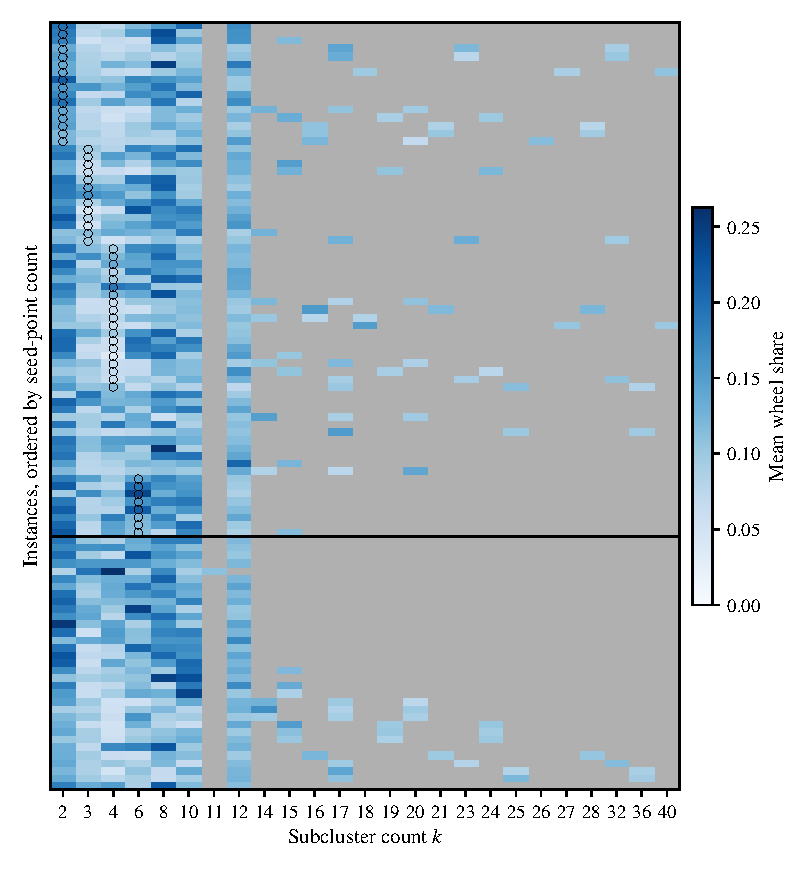
\includegraphics[width=\textwidth]{figures/haos_k_heatmap.pdf}
\caption{Final $k$-Wheel Share, Averaged over the Three Seeds, Supporting Section~\ref{sec:results-haos}. Rows are the 100 XL instances, ordered by the number of customer seed points used to generate them; the random instances, which have none, form the block below the horizontal line. Open circles mark the cell where $k$ equals that seed-point count. Colour runs from zero to the largest share in the figure. Grey cells are arms outside that instance's $k$ domain.}
\label{fig:haos-k}
\end{figure}

\begin{figure}[H]
\centering
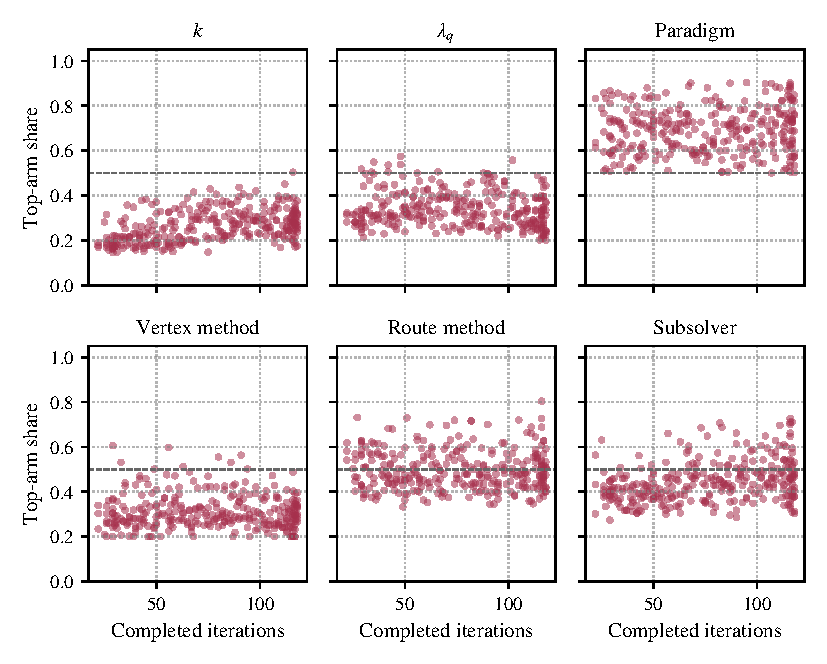
\includegraphics[width=\textwidth]{figures/haos_top_arm.pdf}
\caption{Top-Arm Share of Each HAOS Wheel Against Completed \gls{dri} Iterations, Supporting Section~\ref{sec:results-haos}. The dashed line is a share of one half. A two-arm wheel lies on or above that line on every draw.}
\label{fig:haos-toparm}
\end{figure}

\begin{figure}[H]
\centering
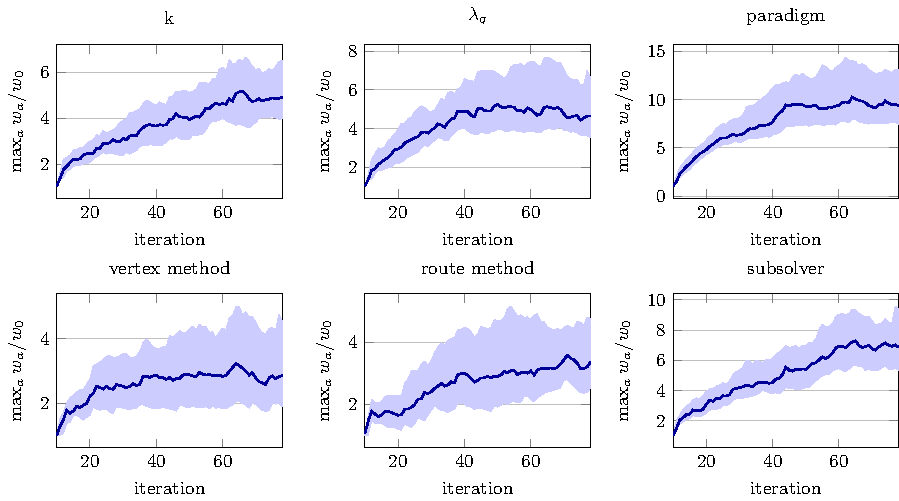
\includegraphics[width=\textwidth]{figures/haos_diag_weight_range.pdf}
\caption{Weight Range of the Six Wheels Against Iteration, Supporting Section~\ref{sec:results-haos}. The curve is the median ratio of the largest weight to $w_0$, and the band is the interquartile range.}
\label{fig:haos-weight-range}
\end{figure}

\begin{figure}[H]
\centering
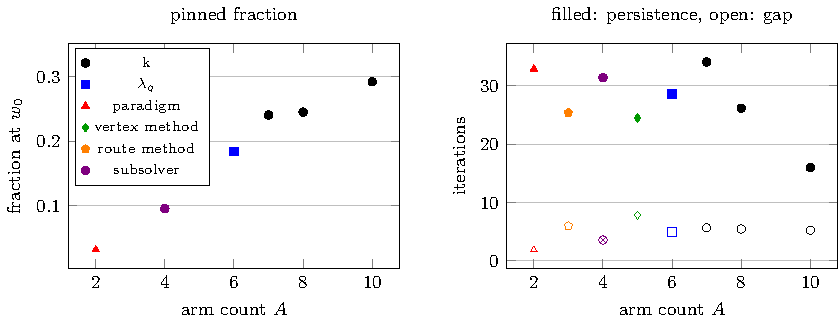
\includegraphics[width=\textwidth]{figures/haos_diag_pinned.pdf}
\caption{Decay-Floor Occupancy and Spell Length, Supporting Section~\ref{sec:results-haos}. The left panel is the fraction of post-warm-up snapshots sitting on the floor. The right panel is the mean spell above the floor and the mean gap before the arm is drawn again.}
\label{fig:haos-pinned}
\end{figure}

\begin{figure}[H]
\centering
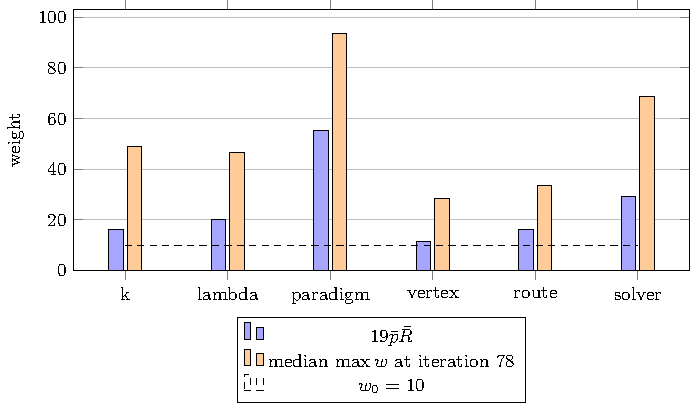
\includegraphics[width=0.92\textwidth]{figures/haos_diag_equilibrium.pdf}
\caption{Observed Median Maximum Weight Against the Interior Fixed Point $19\bar{p}\bar{R}$, Supporting Section~\ref{sec:results-haos}.}
\label{fig:haos-equilibrium}
\end{figure}